%!TEX ROOT=radek-novotny-bp-2017.tex
\chapter{Teoretický základ}
\label{2-teorie}
\section{Eroze}
\subsection{Co je eroze?}
\begin{wrapfigure}{l}{0.43\textwidth}
\vspace{-16pt} \centering
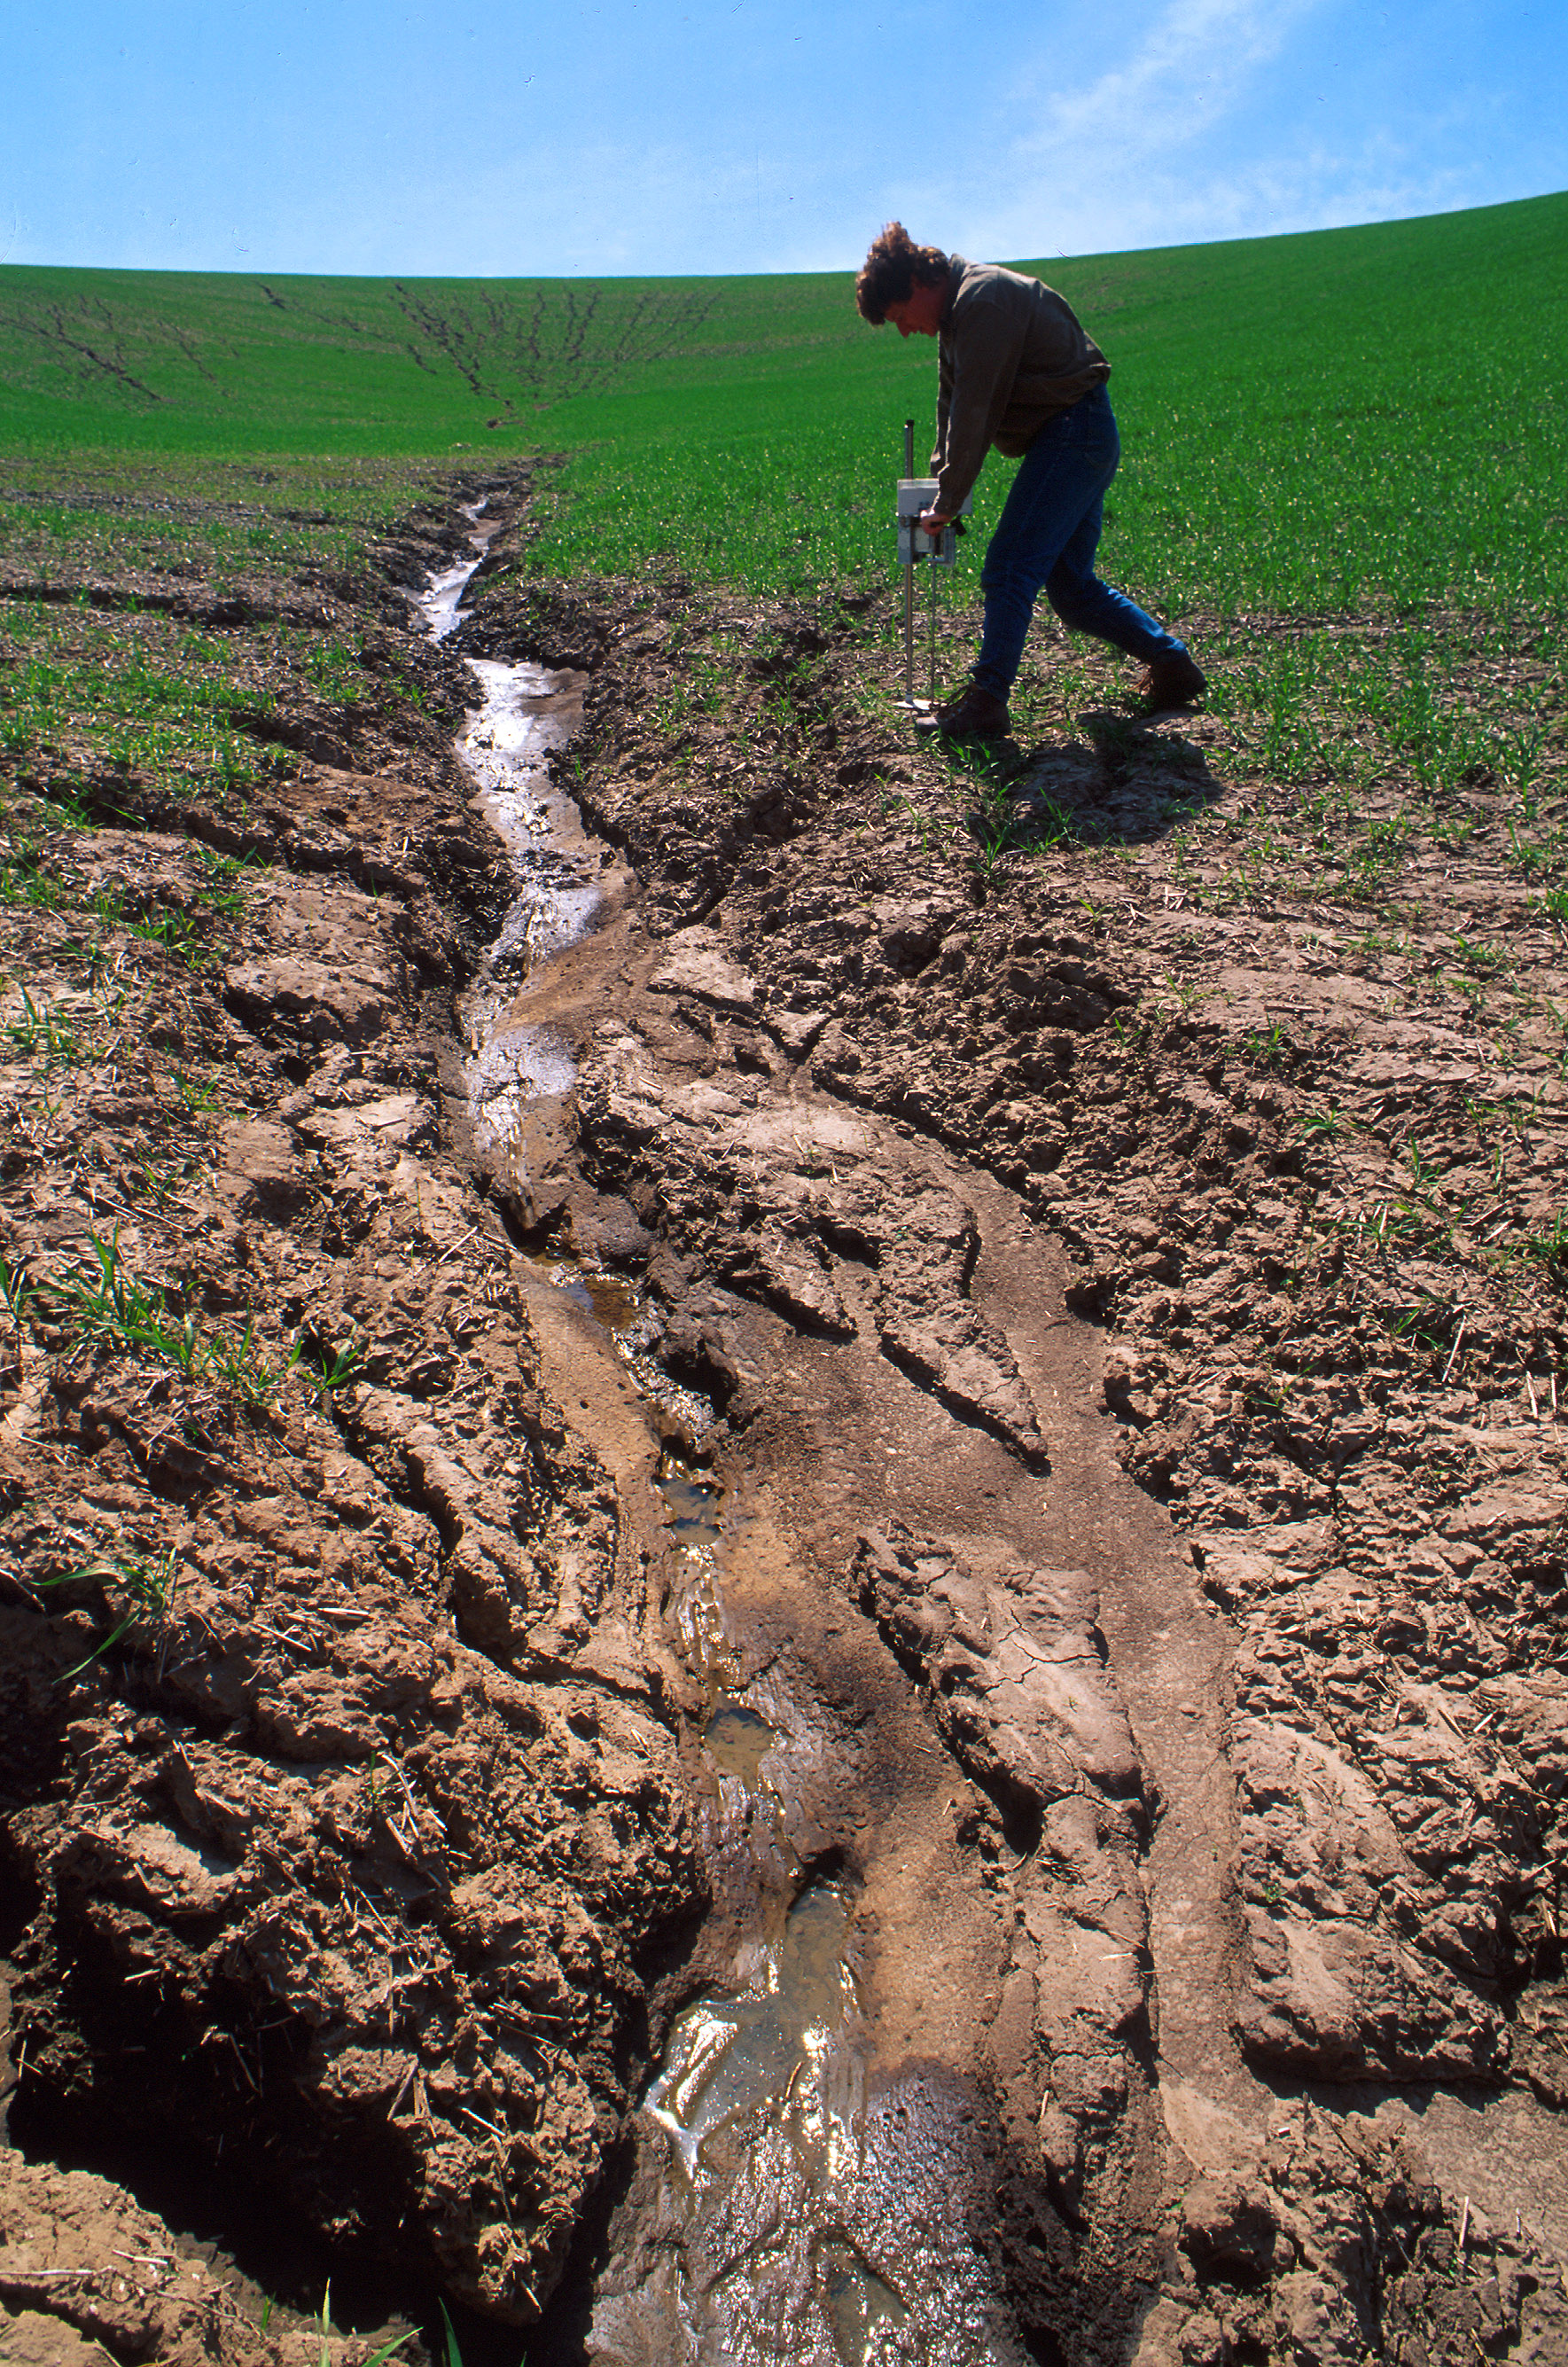
\includegraphics[width=0.43\textwidth]{./pictures/erosion.jpg}
\caption[Ilustrační obrázek eroze]{\label{erosion}Ilustrační obrázek
  eroze zdroj: Wikimedia Commons\cite{wikicommons}}
\vspace{-20pt}
\end{wrapfigure}
Eroze, z latinského „erodere“ – rozhlodávat, je přirozeným přírodním
procesem, během kterého dochází mechanickým působením vnějších faktorů
– vody, větru a sněhu k~rozrušování půdního povrchu, transportu
půdních částic a jejich ukládání na novém místě
(sedimentaci).\cite{Holy1994}

Vliv přirozené neboli geologické eroze není problémem, a naopak je
jedním ze základních procesů tvorby krajiny po milióny let. Dochází
při ní k uvolňování biogenních prvků (např. fosfor, draslík, síra),
jež jsou nezbytné pro život všech organismů a jinak by zůstaly
navázané v horninách. Rychlost geologické eroze je srovnatelná s
rychlostí, kterou je přirozenými procesy vytvářena půda
nová.\cite{Holy1994}

Vlivem antropogenních jevů bohužel nastává tzv. zrychlená půdní eroze,
která má negativní vliv jak na kvalitu půd (zúžení půdního profilu,
snížení obsahu živin, zvýšení štěrkovitosti), jelikož při ní dochází k
odstraňování nejúrodnější složky půdy – ornice, tak na plodiny na ní
pěstované (mechanické poškození, ztráty osiva a~hnojiv). Díky tomu
může na silně erodovaných pozemcích docházet ke ztrátám až 3/4
z~hektarového výnosu. Následná sedimentace půdních částic zanáší vodní
toky, nádrže a při zvýšeném povodňovém průtoku může způsobovat
rozsáhlé škody v intravilánech obcí.\cite{Novotny2014}
\subsection{Rozdělení eroze}
Kromě rozdělení eroze dle intenzity na přirozenou a zrychlenou, je
možné erozi dělit podle činitele, jenž jí způsobuje na erozi vodní,
větrnou a sněhovou.\cite{Holy1994}
\subsubsection{Vodní eroze}
Při vodní (akvatické) erozi dochází k rozrušování zemského povrchu
dopadem vodních kapek, nejsilněji při letních přívalových deštích, kdy
se dopadající voda nestihne vsáknout do půdy a následný povrchový
odtok způsobuje další vymílání a transport půdních částic. Vodní eroze
je v České republice nejčastější a je jí ohroženo více než~50~\%
veškeré orné půdy. Je ovlivněna především sklonem pozemku, délkou
pozemku po spádnici, vegetačním pokryvem a strukturou půdy.

Vodní erozi můžeme dále dělit dle formy odtoku. Jako první probíhá při
dešti plošná eroze (plošný splach), ta je charakteristická
rozrušováním a smyvem půdní hmoty z celého území. Jejím prvním stupněm
je eroze selektivní, při níž jsou povrchovým odtokem odnášeny jemné
půdní částice, na které jsou vázány chemické látky. Tím je způsobena
větší hrubozrnnost a snížení obsahu živin v půdě zasažené
erozí. Naopak půda obohacená smyvem je jemnozrnnější a bohatší na
živiny. Druhý stupeň plošné eroze probíhá při větší kinetické energii
povrchově stékající vody a střídání málo odolných a odolných vrstev,
odtud také název – eroze vrstevná. Projevuje se po celé ploše svahu a
odnáší celé málo odolné vrstvy ornice.

Druhou formou odtoku je výmolová eroze, vznikající postupným
soustřeďováním vody stékající po povrchu a jejím zařezáváním do
půdy. Prvním stádiem je eroze rýžková či brázdová, kdy na povrchu
vznikají úzké rýžky a mělčí širší brázdy, které tvoří na postiženém
území hustou síť. Voda odtékající v soustředěném odtoku má větší
kinetickou energii, čímž transportuje půdu ve větším
rozsahu. Důsledkem stékání rýžek a brázd voda dále získává na síle,
vzniká rýhová eroze. Pokud zesílí mění se v erozi výmolovou či
devastující erozi stržovou, které způsobují hluboké výmoly a
strže.\cite{Novotny2014}
\subsubsection{Větrná eroze}
Druhým nejvýznamnějším typem v ČR je eroze větrná neboli eolická, jež
ohrožuje téměř 10 \% výměry orné půdy. Jedná se území, kde se
vyskytují výsušné větry, pozemky jsou zde sceleny do obrovských
jednotek, na kterých se hospodaří monokulturně a vlivu mechanické síly
větru (abrazi) není bráněno větrolamy, např. oblasti jižní Moravy a
Polabí.

Při větrné erozi dochází k unášení půdních částic různých velikostí,
od velmi jemných zrnek (<0,1 mm), která jsou transportována velmi
snadno ve formě suspenze, často i na velké vzdálenosti a ve větším
množství mohou způsobovat písečné bouře a zákaly atmosféry. Přes
částice střední velikosti (0,1-0,4mm), která představují 50-80\%
celkového objemu přenášeného větrem a způsobují největší škody kolizí
a~rozrušováním vytvořeného půdního agregátu. Po největší zrna (0,5-2
mm), která se pohybují sunutím po povrchu a představují asi 25\%
objemu větrné eroze.\cite{Holy1994}

\subsubsection{Sněhová eroze}
Sněhová eroze transportuje půdní částice obdobně jako eroze vodní,
avšak vyznačuje se určitými specifiky, jedním z nich je zanedbatelný
vliv kinetické energie dopadajících sněhových vloček na rozrušování
povrchu půdy, erozní účinnost sněhu je tedy výhradně při jeho
tání.\cite{Holy1994}

\subsection{Protierozní opatření}
\begin{figure}[H]
    \centering
    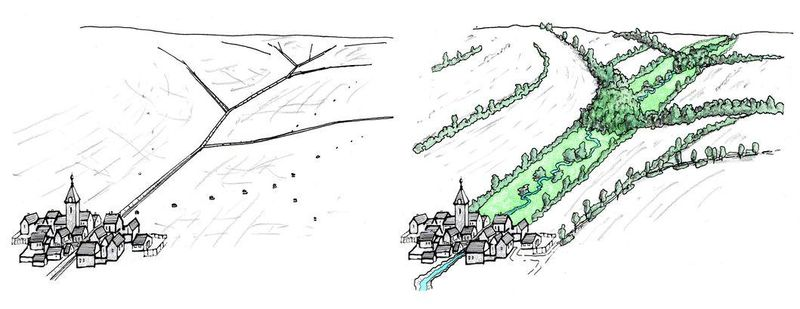
\includegraphics[scale=0.5]{./pictures/protierozni_opatreni.jpg}
      \caption[Ilustrace technického protierozního opatření]{Ilustrace
        technického protierozního opatření, AOPAK ČR\cite{AOPAK} }
      \label{fig:r_faktor_graph}
\end{figure}

Pojem protierozní opatření označuje konkrétní kroky vedoucí k
minimalizaci nega\-tivních dopadů eroze na půdu, vodní toky a nádrže,
intravilán obcí apod. Protierozní opatření dělíme na organizační,
tj. vhodné umístění pěstovaných plodin, pásové střídání plodin nebo
návrhy vegetačních pásů mezi pozemky, agrotechnická (půdoochranné
obdělávání) a technická (příkopy, terasy, protierozní nádrže a
další). Ve většině případů jde o komplex těchto opatření, která se
vzájemně doplňují, aby byly splněny všechny požadavky na ně kladené a
zároveň byly respektovány potřeby zemědělské
výroby.\cite{Holy1994}\cite{janecek2012}

\subsubsection{Organizační protierozní opatření}
Základní organizační protierozní opatření je navržení vhodné velikosti
a tvaru pozem-ku a jeho situování delší stranou po
vrstevnicích. Dodržení tohoto základního pravidla, není vždy
jednoduché, neboť proti sobě působí dva faktory – přírodní, který vede
k vytváření menších pozemků s lepší erozní a ekologickou stabilitou,
a~faktor ekonomický, jenž naopak upřednostňuje tvorbu dostatečně
velkých pozemků pro efektivní využívání zemědělských strojů. Tvar a
velikost pozemku je tedy kompromisem mezi geografickými podmínkami a
požadavky vlastníků (uživatelů) půdy. Obecně se doporučuje navrhování
půdních bloků do 50 ha na rovinných územích a~do~20 ha v územích
členitějších.

Dalším krokem je delimitace (vymezení hranic) druhu pozemků, která
slouží jako funkční a prostorová optimalizace využití pozemků
zemědělského půdního fondu. Ten je rozdělen na ornou půdu, zahrady,
louky, pastviny, vinice, sady a chmelnice. K rozdělení dochází na
základě erozní ohroženosti pozemků, kdy nejohroženější pozemky, které
nemohou být dále využívány jako orná půda, jsou
zatravněny. Umís-těním~trvalého travního porostu by měly být chráněny
také průlehy, ochranné hrázky a břehy vodních toků a nádrží. Je vhodné
umístění liniových pásů travního porostu v drahách výmolové
eroze. Nejúčinnější ochrany proti vodní erozi je dosaženo zalesněním
území, optimálně lesem smíšeným.

Důležitým faktorem je tedy přítomnost vegetačního pokryvu, jehož
význam je nejvyšší v období letních přívalových dešťů. Vegetace chrání
půdu před přímým dopadem dešťových kapek, podporuje vsak vody do půdy
a její kořenový systém pomáhá zvyšovat soudržnost půdy vůči stékající
vodě. Těchto znalostí se využívá při výběru dalších organizačních
opatření, kterými mohou být např. včasný výsev plodin, posunutí
podmítky do období s nižším výskytem přívalových dešťů (tj. na září),
zařazení bezorebně setých meziplodin a v neposlední řadě rozmístění
plodin dle ohroženosti pozemku, kdy pozemky rovinné nebo mírně
sklonité je vhodné využít pro pěstování plodin nedostatečně chránících
půdu před erozí (širokořádkové plodiny) a pro pozemky více ohrožené
volit plodiny s lepším protierozním charakterem nebo pásové střídání
plodin, kdy se střídají pásy plodin chránících půdu (např.~travní
porost, vojtěška, jetel) s plodinami s nižší protierozní účinností
(okopaniny, kukuřice).\cite{janecek2012}

\subsubsection{Agrotechnická protierozní opatření}
Jelikož nejvíce ohrožena erozí je půda bez vegetačního pokryvu, snaží
se agrotechnická protierozní opatření zkrátit období, kdy je půda
obnažena na minimum. Nej\-rizikovějšími obdobími jsou zejména období
tání sněhu a letních přívalových dešťů. Úspěšným prostředkem je cílené
využívání biomasy z meziplodin a posklizňových zbytků, přičemž je
třeba dbát na neomezování možnosti infiltrace vody do půdy.

Mezi nejúčinnější způsoby patří technologie ochranného zpracování
půdy, kdy je místo orby využíváno kypření půdy bez obracení
zpracovávané vrstvy půdy. Ovšem i při orbě lze snížit vliv vodní eroze
dodržením pravidla o orání ve směru vrstevnic, kdy brázdy mohou omezit
povrchový odtok vody. Dále existuje množství dalších technologií, jež
jsou specifické pro pěstované plodiny, jejich přehled je možné najít v
metodice Ochrana zemědělské půdy před
erozí\cite{janecek2012}(str. 60-70).\cite{Holy1994}

\subsubsection{Technická protierozní opatření}
Technické prvky jsou základem protierozní ochrany, a to především tam,
kde smyv z~pozemků má důsledky pro intravilán obce. Jedná se o
převážně liniové prvky, které jsou optimálně rozmisťovány tak, aby
došlo k přerušení délky svahu a rozčlenění pozemků. Dále mají vliv na
agrotechnické opatření, kdy usměrňují směr obdělávání pozemků a způsob
hospodaření jejich uživatelů. Vhodná je i jejich kombinace s
organizačními opatřeními, kdy po rozdělení svahu liniovými opatřeními
jsou do nově vymezených pásů umístěny plodiny s různou protierozním
povahou. V neposlední řadě je jejich funkce i ekologického a krajině
estetického charakteru. Technická protierozní opatření jsou navrhována
během pozemkových úprav a patří mezi ně průlehy, příkopy, hrázky,
meze, ochranné nádrže, stabilizování drah soustředného odtoku a
terasování. Způsoby navrhování zmiňovaných opatření lze dohledat
v~meto-dice Ochrana zemědělské půdy před
erozí\cite{janecek2012}(str. 70-90). Dále lze čerpat z
\cite{Kadlec2014}\cite{Novotny2014}.
\newpage
\section{Historie}
\subsection{Počátky výzkumu eroze}
Výzkumem eroze se začali zabývat vědci v USA začátkem 20. století,
jednou z~významných osobností při prvních krocích výzkumu byl Hugh
Bennett, který začal pozorovat zvýšenou erozi na zemědělské půdě a
její vliv na výnos. Bennett na tento rostoucí problém veřejně
upozorňoval, do většího povědomí se však ochrana zemědělské půdy
dostala až na přelomu 20. a 30. let v souvislosti s mohutnými
prachovými bouřemi (tzv. Dust Bowl, Dirty Thirties).\cite{usda_ars}
\begin{figure}[H]
    \centering 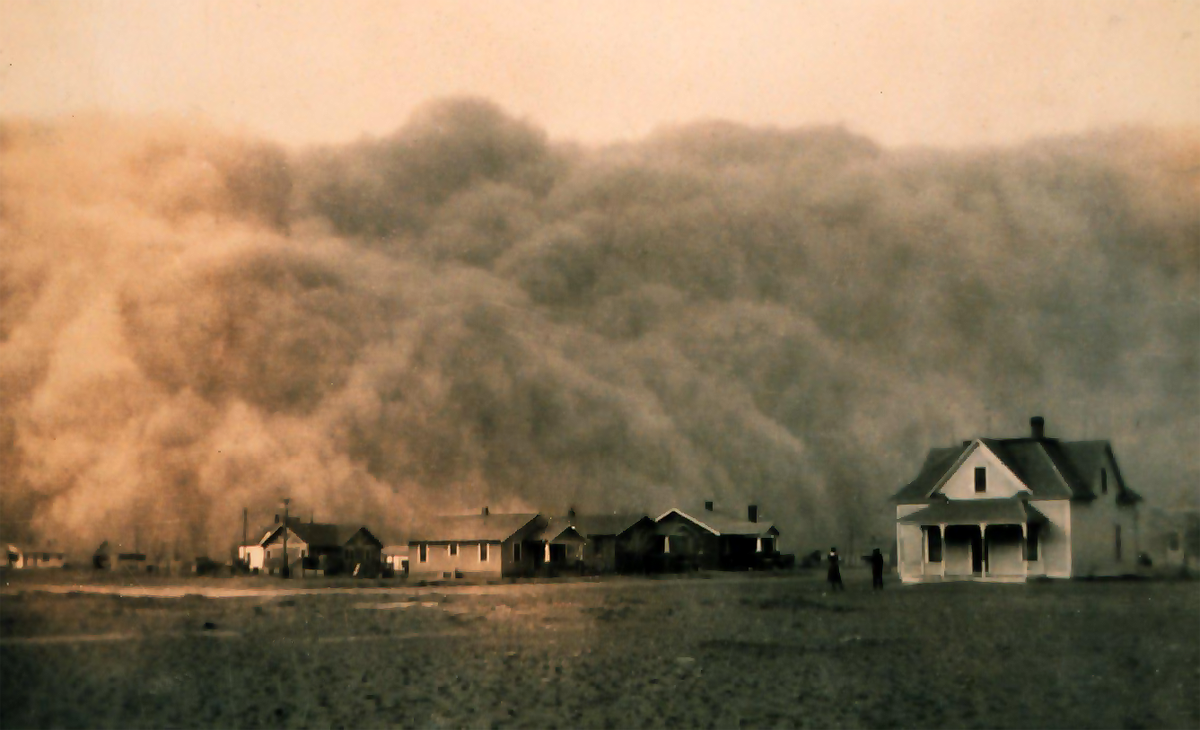
\includegraphics[scale=0.7]{./pictures/Dust_bowl.png}
      \caption[Foto bouře v oblasti Dust Bowl z roku 1935]{Foto bouře
        v oblasti Dust Bowl z roku 1935, zdroj: Wikimedia
        Commons\cite{wikicommons}}
      \label{fig:dust_bowl}
\end{figure}

\paragraph{Dust Bowl,} slovní spojení, jež bylo původně použito pro oblast vzniku prachových
bouří - Velkých planin a následně se stalo synonymem i pro období
30. let (proto také druhý název Dirty Thirties), kdy se bouře
objevovaly. Příčinou byla rychlá změna suchých prérií s nízkým
srážkovým úhrnem (místy pod 250 mm/rok) na zemědělskou půdu. Tuto
změnu umožnilo rozšíření zemědělských strojů, zejména traktorů, díky
kterým mohla být na rozsáhlém území využita hluboká orba, kterou byla
zničena původní vegetace chránící půdní povrch. Místo původních travin
byla na většině území vysazena pšenice, přičemž nebylo dodržováno ani
střídavé hospodaření.

Ve spojení s nulovou ochranou půdy došlo tímto způsobem zemědělství v
obdobích sucha k proměně půdy v prach, který byl unášen větrem a
vytvářel mohutná prachová oblaka devastující krajinu. Erozí zasáhla
okolo 100 milionů akrů půdy (v~roce 1934 bylo bouří zasaženo dokonce
východní pobřeží USA včetně New Yorku), zanechala bez domova téměř 500
tisíc lidí a způsobila stěhování až 3,5 milionu lidí ze zasažené
oblasti, čímž se jednalo o největší migrační vlnu v historii
USA. Touto katastrofou byla dále prohloubena Velká hospodářská krize.

První reakcí bylo v roce 1929 zřízení deseti výzkumných stanic, ve
kterých byla na tzv. jednotkových pozemcích (délka 22,13 m, sklon
9$\%$, trvalý úhor, obdělávání ve směru sklonu) pozorována eroze a
měřen smyv. Z měření byla regresní analýzou odvozeny faktory
ovlivňující erozi a účinnost ochranných opatření. Další krok učinil v
roce 1932 nově zvolený americký prezident Franklin Roosevelt, který v
rámci opatření proti trvající hospodářské krizi zřídil úřad zabývající
se půdní erozí (SES – Soil Erosion Service), v čele kterého stanul
H. Bennett. Tento úřad začal učit farmáře šetrnějším metodám
hospodaření, budovat velké množství protierozních opatření, při čemž
zaměstnával dělníky zasažené ekonomickou depresí, a samozřejmě
pokračoval ve výzkumu eroze.\cite{Bonnifield1979}\cite{Egan2006}

\subsection{Vývoj USLE}
\begin{figure}[H]
    \centering 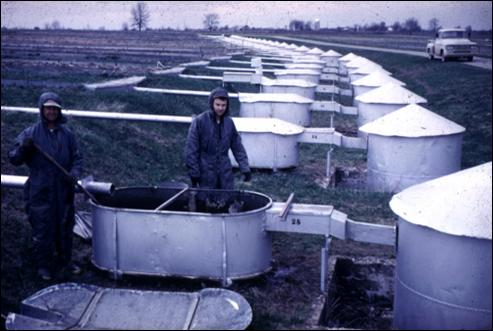
\includegraphics[scale=0.85]{./pictures/unit_plots.jpg}
      \caption[Foto jednotkových pozemků v Missouri v 50. letech]{Foto
        jednotkových pozemků v Missouri v 50. letech, zdroj: USDA
        ARS\cite{usda_ars}}
      \label{fig:unit_plots}
\end{figure}
Díky studiím z výzkumných stanic, které postupně vznikaly, bylo
shromážděno velké množství informací, které byly dále využity pro
výpočty erozního smyvu. Vývoj matematických rovnic pro odhad množství
půdní eroze a vliv ochranných opatření začal v druhé polovině
30. let. První empirický model(\ref{zing1940}) pro odhad průměrné
roční ztráty půdy způsobené vodní erozí publikoval v roce 1940
A. W. Zingg. Jeho rovnice zahrnovala vliv sklonu pozemku a jeho
délku. Konstanty byly určovány pro kukuřičný pás (Corn Belt), hlavní
zemědělskou oblast USA.\cite{ZINGG1940}
\begin{align}
   \label{zing1940} G=L^{0,6}\cdot S^{1,4}\cdot C
\end{align}
\hspace*{2cm}$G \cdots$ průměrná roční ztráta půdy\\
\hspace*{2cm}$L \cdots$ délka svahu \\
\hspace*{2cm}$S \cdots$ sklon svahu \\
\hspace*{2cm}$C \cdots$ koeficient zahrnující ostatní faktory\\

Tento model v roce 1941 rozšířil D. D. Smith, který do rovnice
(\ref{smith1941}) zahrnul vliv technických protierozních
opatření. Smith jako první využil její výsledky využil k určení
maximální délky svahu na specifickém území a stanovení metod
ochrany.\cite{Smith1941}
\begin{align}
   \label{smith1941} G=L^{\frac{3}{5}}\cdot S^{\frac{7}{5}}\cdot P\cdot C
\end{align}
\hspace*{2cm}$G \cdots$ průměrná roční ztráta půdy\\
\hspace*{2cm}$L \cdots$ délka svahu \\
\hspace*{2cm}$S \cdots$ sklon svahu \\
\hspace*{2cm}$P \cdots$ faktor protierozních opatření \\
\hspace*{2cm}$C \cdots$ koeficient zahrnující ostatní faktory \\

Tato rovnice byla G. M. Browning použita pro sestavení empirického
modelu pro stát Iowa (\ref{browning}), kde jsou poprvé zahrnuty
geologické faktory půdy a agrotechnických opatření.\cite{browning1947}
\begin{align}
   \label{browning} G=10\cdot\left( K^{\prime}\cdot O^{\prime}\cdot  L^{\prime}\cdot S^{\prime}\cdot C^{\prime}\cdot P^{\prime} \right)
\end{align}
\hspace*{2cm}$G \cdots$ průměrná roční ztráta půdy\\
\hspace*{2cm}$K^{\prime} \cdots$ faktor erodovatelnosti půdy \\
\hspace*{2cm}$O^{\prime} \cdots$ faktor geologického podkladu \\
\hspace*{2cm}$L^{\prime} \cdots$ délka svahu \\
\hspace*{2cm}$S^{\prime} \cdots$ sklon svahu \\
\hspace*{2cm}$C^{\prime} \cdots$ faktor vegetačního pokryvu \\
\hspace*{2cm}$P^{\prime} \cdots$ faktor protierozních opatření \\

V roce 1947 Musgrave publikoval první erozní
model(\ref{musgrave1947}), který zahrnoval vliv přívalového deště. V
této rovnici byly také překlasifikovány hodnoty faktorů pro kukuřičný
pás.\cite{MUSGRAVE1947}

\begin{align}
   \label{musgrave1947} G=K\cdot C\cdot L^{0,35}\cdot S^{1,35}\cdot R^{1,75}
\end{align}
\hspace*{2cm}$G \cdots$ průměrná roční ztráta půdy\\
\hspace*{2cm}$K \cdots$ geologický faktor eroze půdy \\
\hspace*{2cm}$C \cdots$ faktor vegetačního pokryvu \\
\hspace*{2cm}$L \cdots$ délka svahu \\
\hspace*{2cm}$S \cdots$ sklon svahu \\
\hspace*{2cm}$R \cdots$ úhrn deště s periodicitou 0,5 za 30 minut \\
\begin{figure}[H]
    \centering
    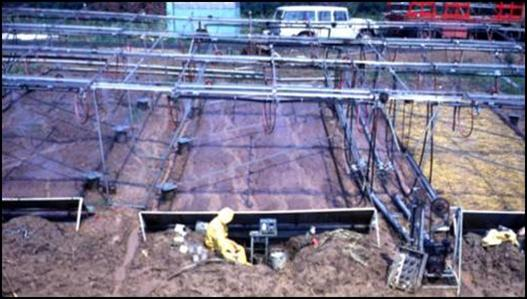
\includegraphics[scale=0.85]{./pictures/unit_plots2.jpg}
      \caption[Foto jednotkových pozemků v Indianě (1968)]{Foto
        jednotkových pozemků v Indianě (1968), zdroj: USDA
        ARS\cite{usda_ars}}
      \label{fig:unit_plots}
\end{figure}
V roce 1954 na Purdue University, která měla v té době vedoucí
postavení v~oblasti výpočetních technologií, vzniklo pod vedením
W. H. Wischmeier centrum pro shromažďování dat o půdní erozi (Soil
Loss Data Center). Přístup k nejmodernějším technologiím dovolil
zrychlit analyzování velkého množství dat (v letech 1940-1965 přes
10~000 zmonitorovaných smyvů ročně), jež byly shromažďovány od
30. let. Výsledkem byla v roce 1965 první kompletní publikace
vytvořená týmem pod vedením Wischmeier a Smith, která byla ještě
zpřesněna dalším výzkumem a upravena do současné formy(\ref{usle1978})
publikované v roce 1978.\cite{usle1978}

\begin{align}
   \label{usle1978} G=R\cdot K\cdot L\cdot S\cdot C\cdot P
\end{align}
\hspace*{2cm}$G \cdots$ průměrná roční ztráta půdy $\left( t\cdot
ha^{-1}\cdot rok^{-1} \right)$\\
\hspace*{2cm}$R \cdots$ faktor erozní účinnosti deště \\
\hspace*{2cm}$K \cdots$ geologický faktor eroze půdy \\
\hspace*{2cm}$L \cdots$ faktor délky svahu \\
\hspace*{2cm}$S \cdots$ faktor sklonu svahu \\
\hspace*{2cm}$C \cdots$ faktor vegetačního pokryvu \\
\hspace*{2cm}$P \cdots$ faktor protierozních opatření \\

\subsection{Modifikace USLE}
\subsubsection{RUSLE}
V roce 1997 byla publikována Revidovaná univerzální rovnice ztráty
půdy (Revised Universal Soil Loss Equation), ta byla odvozena na
základě revize, prověření a aktualizace USLE. Došlo
zde k významné změně způsobu určení erozních faktorů (např. zpřesnění
časového průběhu hodnot R faktoru v patnáctidenním intervalu,
zpřesnění časového průběhu K faktoru v důsledku zhutňování povrchu a
rozpadu půdních agregátů srážkami či obhospodařováním, nové vztahy pro
LS faktor). Výhodou využití RUSLE je tedy přesnější určení
%%% ML: to zavani zastaralosti zdroje, ktery jste pouzil
%%% RN: zrejme zbytecne, odstraneno
erozního modelu. Nevýhodou je nutnost většího množství vstupních
dat.\cite{rusle1997}
\subsubsection{MUSLE}
Druhou významnou úpravou je Modifikovaná univerzální rovnice ztráty
půdy (Modified Universal Soil Loss Equation), která zahrnuje
transportní činitele během erozního procesu a stanovuje množství
splavenin z přívalového deště v povodí do velikosti
15~km$^{2}$.\cite{musle1945}

%%% ML: tato kapitola se tyka ciste CR, je to tak? Pokud ano, tak by
%%% to mel zohlednit jeji nazev
%%% RN: CR se tyka pouze prvni polovina prvniho odstavce, zbytek by
%%% mel platit obecne, nazvem a strukturu kapitoly jeste promyslim
\newpage
\subsection{Současný stav}
USLE je v současnosti používána pro výpočet dlouhodobé eroze ve
%%% ML: opravdu jedinou?
%%% RN: pro vypocet dlouhodobe eroze ano, dale existuji simulacni
%%% modely pro vypocet eroze kratkodobe, zrejme tuto kapitolu ale
%%% jeste uppravim
většině států světa a je jedinou doporučenou metodou v ČR (Metodika
VÚMOP\cite{janecek2012}), existují k ní rozsáhlá katalogová data. Jsou
vytvořeny postupy pro její výpočet v softwarech GIS a je přímo
implementována pro automatické zpracování programy jako jsou USLE2D či
modulem Eroze pro Atlas DMT. Ovšem i přes úpravy a postupné zlepšení
schopnosti odhadu dlouhodobé ztráty půdy je USLE i další zmíněné
metody empirické, tedy založené na využití koeficientů získaných při
pozorování v terénu (na jednotkových pozemcích). Jejich přesnost je
tedy závislá na přesnosti klasifikace jednotlivých faktorů pro
specifickou situaci.

V posledních letech je snaha omezit zavedený empirický základ při
posuzování erozních procesů a nahradit ho kvalitnějšími simulačními
metodami. Cílem této změny je hodnotit důsledky eroze nejen vůči
zemědělské půdě, ale i vůči jiným ekologickým celkům (např. vodní
toky, nádrže) a také řešení eroze na kratším časovém horizontu.  K
vývoji a zdokonalování simulačních modelů přispívá rozvoj výpočetní
techniky, geografických informačních systémů a rozšiřování znalostí v
dané oblasti.\cite{janecek2012}
\begin{figure}[H]
    \centering
    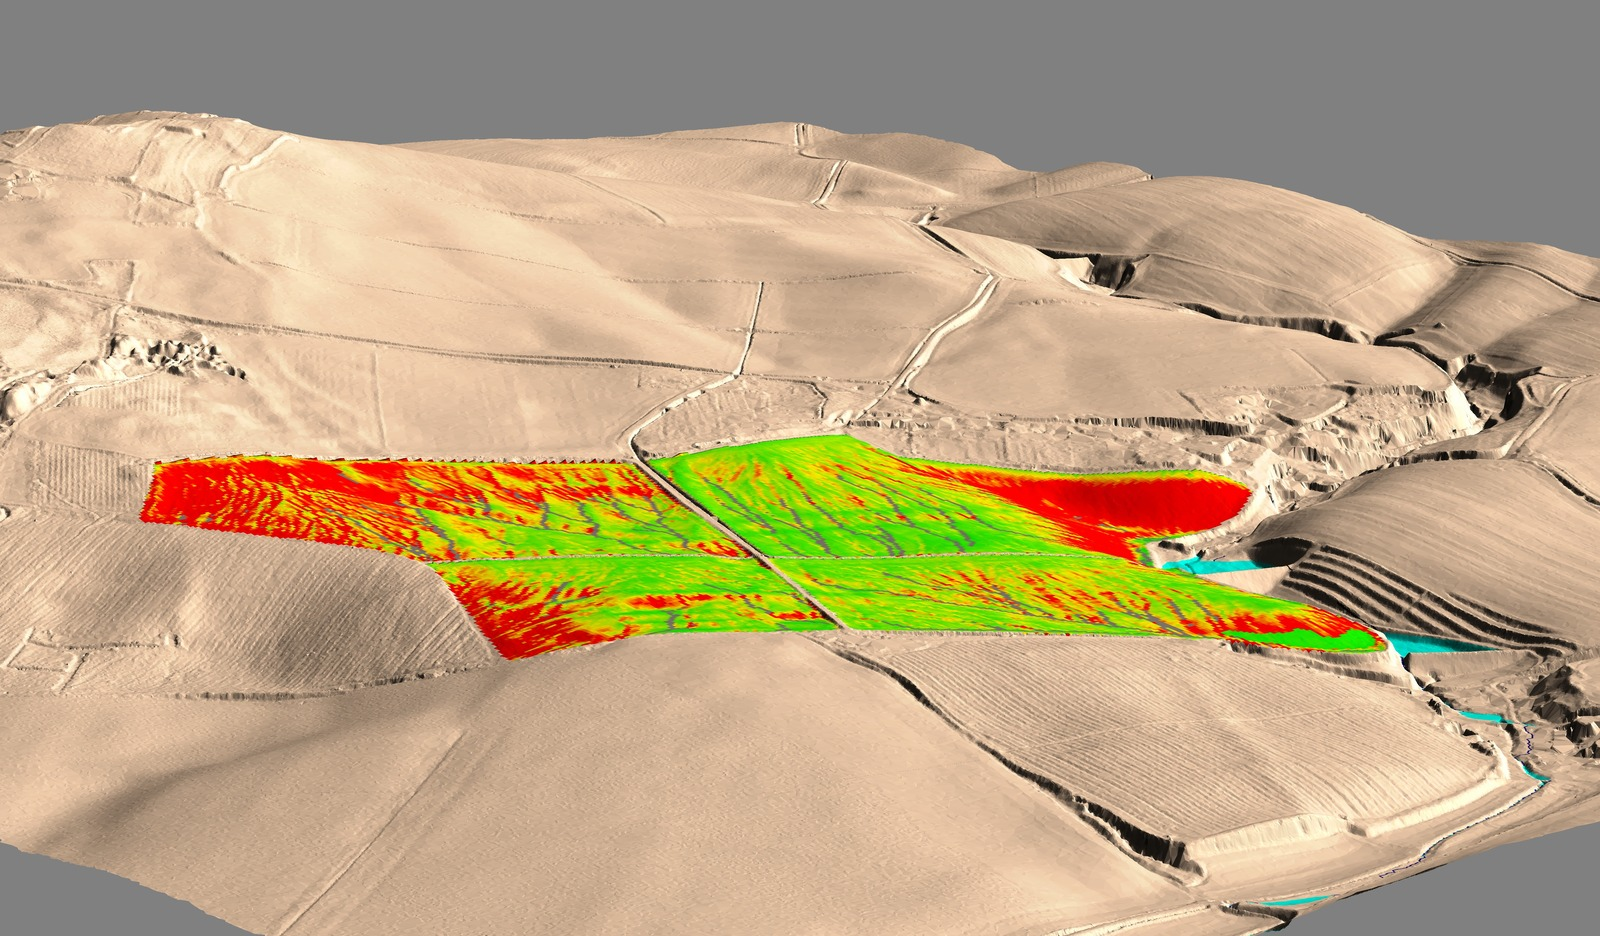
\includegraphics[scale=0.25]{./pictures/atlas_eroze.jpg}
      \caption[Ukázka z výpočtu v GIS aplikaci Eroze pro Atlas
        DMT]{Ukázka z výpočtu v GIS aplikaci Eroze pro Atlas DMT,
        zdroj: Atlas DMT\cite{atlas_e}}
      \label{fig:atlas_eroze}
\end{figure}

\section{Univerzální rovnice ztráty půdy}
\subsection{Faktor erozní účinnosti přívalového deště (R)}
I přesto, že významnější rýhová eroze je pozorována zejména po
neobvykle silných přívalových deštích, během výzkumu byla prokázána
nutnost při odhadu průměrné roční ztráty půdy uvažovat i deště se
střední intenzitou. Pro \zk{usle} byl použit vztah odvozený
Wischmeierem\cite{Wischmeier1959}, který nejlépe aproximoval hodnoty
působení faktoru deště získané z jednotkových pozemků při stálosti
ostatních faktorů. V tomto vztahu nebyl zahrnut smyv při zavlažování
či působení sněhové eroze (tání, obleva), která může být významná v
horských oblastech v jarním období a pro její určení je nutné využít
speciální vztah.

Pro určení srážkového erozního faktoru jsou využity deště oddělené od
sebe alespoň 6~hodin, přičemž nejsou uvažovány ty s úhrnem nižším než
12,5~mm~(0,5 palce) nebo 6,25~mm~(0,25 palce) za~15 minut, jelikož
jejich vliv je zanedbatelný.

Dle definice je hodnota R (v anglické literatuře též označováno jako
parametr EI) dána součinem kinetické energie deště s jeho maximální
30minutovou intenzitou~(\ref{r_factor_1}). Jelikož se ukázalo, že
samotná energie nedostatečně popisuje destruktivní vliv dopadajících
kapek na půdní povrch.\cite{usle1978}
\begin{align}
   \label{r_factor_1} R=E\cdot  \frac{i_{30}}{100}
\end{align}
\hspace*{2cm}$R \cdots$ faktor erozní účinnosti deště $\left( MJ\cdot
ha^{-1}\cdot cm \cdot h^{-1} \right)$\\
\hspace*{2cm}$E \cdots$ celková kinetická energie deště $\left( J\cdot
m^{-2} \right)$\\
\hspace*{2cm}$i_{30} \cdots$ maximální 30minutová intenzita deště
$\left( cm\cdot h^{-1} \right)$\\

Celková kinetická energie deště je sumou ze všech úseků
deště~(\ref{r_factor_2}), kdy jednotlivá kinetická energie závisí na
intenzitě a úhrnu~(\ref{r_factor_3}).\cite{usle1978}
\begin{align}
   \label{r_factor_2} E=\sum_{i=1}^n E_{i}
\end{align}
\begin{align}
   \label{r_factor_3} E_{i}=\left( 206+87 \log i_{si} \right) \cdot H_{si}
\end{align}
\hspace*{2cm}$E_{i} \cdots$ kinetická energie i-tého úseku deště
$\left( J\cdot m^{-2} \right)$\\
\hspace*{2cm}$i_{si} \cdots$ intenzita i-tého úseku deště $\left(
cm\cdot h^{-1} \right)$\\
\hspace*{2cm}$H_{si} \cdots$ úhrn v i-tém úseku deště $\left( cm
\right)$\\

Na základě vypočtených hodnot byla pro USA vytvořena mapa zobrazující
pomocí izolinií průměrné hodnoty R faktoru. \cite{usle1978} V ČR je
dle platné metodiky doporučeno využívat průměrnou
hodnotu.\cite{janecek2012}

Ta byla původně stanovena na 20 $MJ\cdot ha^{-1}\cdot cm \cdot
h^{-1}$. Vycházela z měření na třech stanicích a úhrn dešťů, jež
byly použity pro výpočet, byly sníženy o 12,5 mm. Po použití dat z více
stanic a provedení lepšího metodického rozboru erozní účinnosti deště
bylo určeno, že R faktor se na většině zemědělsky využívaném území ČR
pohybuje mezi hodnotami 30 až 45 $MJ\cdot ha^{-1}\cdot cm \cdot
h^{-1}$., pročež je doporučeno volit tento faktor jako konstantní
hodnotu 40 $MJ\cdot ha^{-1}\cdot cm \cdot h^{-1}$.\cite{janecek2012}

Regionalizovaná mapa(obr. \ref{fig:r_faktor}) s nejnovějšími hodnotami
R faktoru lze najít na serveru SOWAC-GIS.\cite{sowac}

\begin{figure}[H]
    \centering 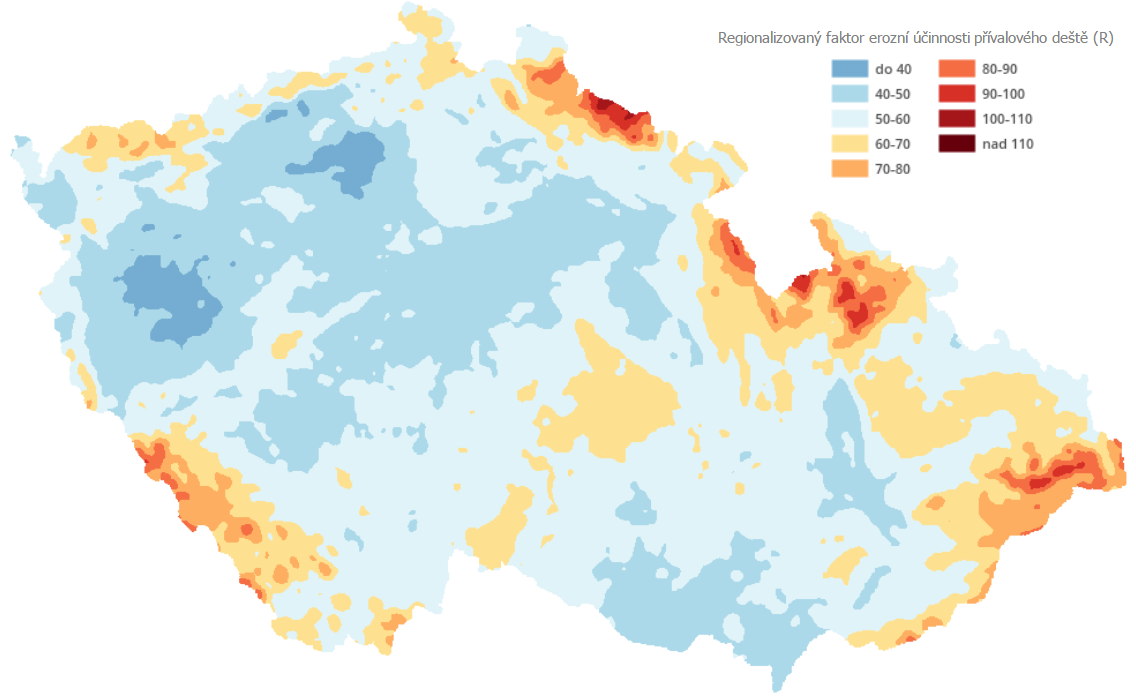
\includegraphics[scale=0.5]{./pictures/r_factor.png}
      \caption{Regionalizované rozdělení faktoru R}
      \label{fig:r_faktor}
\end{figure}

\subsection{Faktor struktury půdy (K)}
Faktor erodovatelnosti půdy udává náchylnost půdy, jako samotné
matérie, k erozi. Měření probíhalo na jednotkových pozemcích
ponechaných ladem, přičemž ostatní faktory (kromě faktoru R, kterým
byla celková eroze vydělena) byly rovny jedné. Jedná se o
komplikovanou proměnou závislou na struktuře, textuře a dalších
fyzic\-kých i chemických vlastnostech zeminy.\cite{usle1978}

První možností, jak faktor erodovatelnosti můžeme určit, je přibližně
podle hlavní půdní jednotky (HPJ) bonitačního půdního systému
(tab. \ref{hpj_k}) nebo Taxonomického klasifikačního systému půd
ČR\cite{Nemecek2001}, jež je rovněž tabelován\cite{janecek2012}. Jedná
se o obdobné řešení jako v původním modelu pro USA, kdy byly vybrány
hlavní půdní typy, pro které byl K faktor určen.\cite{usle1978}

\begin{table}[hbt]
\begin{center}
\catcode`\-=12
    \noindent\begin{tabular}{|*{8}{c|}} \hline \bf HPJ & \bf K & \bf
    HPJ & \bf K & \bf HPJ & \bf K& \bf K & \bf HPJ\\ \hline \bf 1
    &0,41 &\bf 19&0,33 &\bf 36&0,26 &\bf 54&0,40 \\ \hline \bf 2 &0,46
    &\bf 20&0,28 &\bf 37&0,16 &\bf 55&0,25 \\ \hline \bf 3 &0,35 &\bf
    21&0,15 &\bf 38&0,31 &\bf 56&0,40 \\ \hline \bf 4 &0,16 &\bf
    22&0,24 &\bf 40&0,24 &\bf 57&0,45 \\ \hline \bf 5 &0,28 &\bf
    23&0,25 &\bf 41&0,33 &\bf 58&0,42 \\ \hline \bf 6 &0,32 &\bf
    24&0,38 &\bf 42&0,56 &\bf 59&0,35 \\ \hline \bf 7 &0,26 &\bf
    25&0,45 &\bf 43&0,58 &\bf 60&0,31 \\ \hline \bf 8 &0,49 &\bf
    26&0,41 &\bf 44&0,56 &\bf 61&0,32 \\ \hline \bf 9 &0,60 &\bf
    27&0,34 &\bf 45&0,54 &\bf 62&0,35 \\ \hline \bf 10&0,53 &\bf
    28&0,29 &\bf 46&0,47 &\bf 63&0,31 \\ \hline \bf 11&0,52 &\bf
    29&0,32 &\bf 47&0,43 &\bf 64&0,40 \\ \hline \bf 12&0,50 &\bf
    30&0,23 &\bf 48&0,41 &\bf 67&0,44 \\ \hline \bf 13&0,54 &\bf
    31&0,16 &\bf 49&0,35 &\bf 68&0,49 \\ \hline \bf 14&0,59 &\bf
    32&0,19 &\bf 50&0,33 &\bf 70&0,41 \\ \hline \bf 15&0,51 &\bf
    33&0,31 &\bf 51&0,26 &\bf 71&0,47 \\ \hline \bf 16&0,51 &\bf
    34&0,26 &\bf 52&0,37 &\bf 72&0,48 \\ \hline \bf 17&0,40 &\bf
    35&0,36 &\bf 53&0,38 &\bf 73&0,48 \\ \hline \bf 18&0,24 & & & & &
    & \\ \hline
    \end{tabular}\\
    \vspace{10px} Vynechané HPJ nemají K faktor určen kvůli nedostatku
    dat.
  \caption[Hodnoty K faktoru pro jednotlivé HPJ]{Hodnoty K faktoru pro
    jednotlivé HPJ dle metodiky \cite{janecek2012}.}
  \label{hpj_k}
\end{center}
\end{table}
\FloatBarrier Druhou a přesnější metodou, je použití definovaného
vztahu, který je podrobně rozebrán Janečkem\cite{janecek2012} na
str. 13, či použití z něho odvozeného
nomogramu(obr.\ref{fig:k_faktor}). Ovšem pro toto věrnější určení K
faktoru je nezbytné mít k dispozici výsledky rozborů půdy z daného
území.\cite{janecek2012}

\begin{figure}[H]
    \centering
    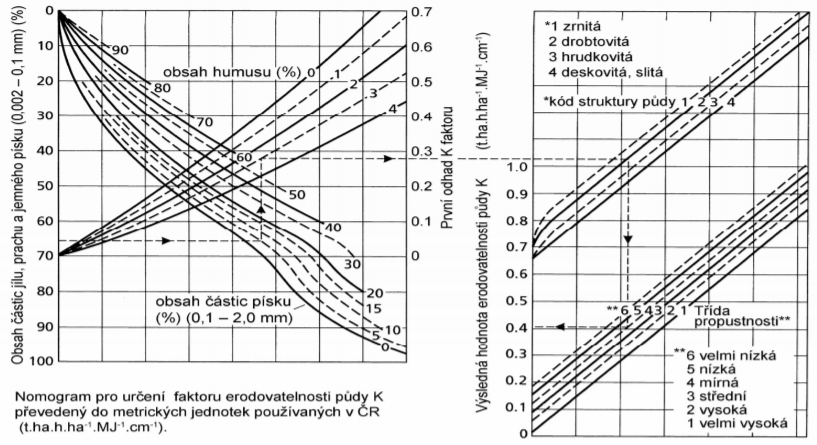
\includegraphics[scale=0.85]{./pictures/k_faktor_nomogram.png}
      \caption[Nomogram pro stanovení K faktoru]{Nomogram pro
        stanovení K faktoru (zdroj: Janeček\cite{janecek2012})}
      \label{fig:k_faktor}
\end{figure}
\subsection{Topografický faktor (LS)}
I přestože faktory sklonu a délky svahu byly zkoumány odděleně a oba
jsou reprezentovány vlastní rovnicí pro výpočet eroze, jsou často
uváděny jako jeden tzv. topografický faktor.\cite{usle1978}

Původní a dodnes využívanou metodou pro jeho určení je výpočet v
tzv. reprezentativních odtokových drahách, které jsou voleny od místa
vzniku povrchového odtoku, tedy rozvodnice či hrany pozemku, pokud je
tento pozemek erozně izolován, po místo, kde se plošná eroze mění v
soustředný odtok. Dále už není možné pro výpočet eroze použít metodu
USLE, jelikož slouží pouze pro výpočet plošné eroze. Také není
doporučeno, aby délka rozvodnice přesáhla 400 m, jelikož výsledky USLE
pro větší délky nejsou ověřeny.\cite{janecek2012}

\subsubsection{Faktor délky svahu - L} 
Při použití reprezentativních odtokových drah se faktor L určí pomocí
vztahu (\ref{l_faktor}), který byl definován v RUSLE\cite{rusle1997} a
jehož výsledkem je poměr ztráty půdy na jednotku plochy svahu ke
ztrátě na jednotkovém pozemku (délka 22,13 m, sklon
9\%).\cite{janecek2012}
\begin{align}
   \label{l_faktor} L=\left( \frac{l}{22,13} \right)^m
\end{align}
\hspace*{2cm}$l \cdots$ horizontální projekce nepřerušené délky svahu
$\left( m \right)$ \\
\hspace*{2cm}$m \cdots$ exponent náchylnosti svahu ke vzniku rýžkové
eroze dle sklonu svahu, tabelovaný v RUSLE\cite{rusle1997} \\
\subsubsection{Faktor sklonu svahu - S} 
Obdobně je tomu u vztahu pro faktor sklonu svahu, jež se liší pro
sklony nižší než 9\% (\ref{s_faktor1}) a slony větší
(\ref{s_faktor2}). Tyto vztahy byly taktéž uvedeny v
RUSLE\cite{rusle1997}.
\begin{align}
   \label{s_faktor1} S=10,8\cdot\sin\Theta + 0,03
\end{align}
\vspace{-40pt}
\begin{align}
   \label{s_faktor2} S=16,8\cdot\sin\Theta - 0,50
\end{align}
\hspace*{2cm}$\Theta \cdots$ úhel sklonu svahu $\left( rad \right)$

\subsubsection{Výpočet faktoru LS s využitím GIS} 
Druhou metodou je výpočet LS faktoru s pomocí GIS, kdy je výpočet
proveden pro mikropovodí v každém pixelu. Pro výpočet LS faktoru
existuje celá řada definovaných vztahů, jejichž porovnáním se zabýval
Krása\cite{Krasa2010}. Pro české podmínky se používá s dostatečnou
přesností rovnice(\ref{ls_faktor}) odvozená
Mitášovou\cite{Mitasova1998}.\cite{Dostal2014}
\begin{align}
   \label{ls_faktor} LS_{x,y}=\left( m+1 \right)\cdot\left(\frac{A_{x,y}}{22,13}\right)^m \cdot \left(\frac{\sin b_{x,y}}{0,09}\right)^n
\end{align}
\hspace*{2cm}$LS_{x,y} \cdots$ LS faktor pixelu o souřadnicích x, y
\\ \hspace*{2cm}$A \cdots$ jednotková zdrojová plocha na vstupu do
buňky $\left( m^2\cdot bm^{-1} \right)$ \\
\hspace*{2cm}$b \cdots$ sklon buňky $\left( rad \right)$ \\
\hspace*{2cm}$m \cdots$ kalibrační parametr, obvykle 0,6\\
\hspace*{2cm}$n \cdots$ kalibrační parametr, obvykle 1,3\\

Při výpočtu jsou klíčovými faktory určení rastru zdrojových ploch,
přičemž by neměl být použit model s jednosměrným odtokem, a zohlednění
přerušení povrchového odtoku.\cite{Krasa2010}

\subsection{Faktor ochranného vliv vegetace (C)}
Vegetační faktor se uplatňuje především přímou ochranou půdy před
dopadajícími dešťovými kapkami, dále zpomaluje povrchový odtok,
zpevňuje půdu kořenovým systémem a nepřímo se vlivem vegetace mění i
vlastnosti půdy.

Účinnost ochranného vlivu vegetace se projevuje zejména v období
zvýšeného výskytu přívalových dešťů
(obr. \ref{fig:r_faktor_graph}). Nejdokonaleji půdu chrání les,
vysokou protierozní účinnost mají též traviny a
jeteloviny. Nedostatečně půdu chrání širokořádkové plodiny jako je
kukuřice nebo okopaniny a téměř vůbec není půda chráněna na vinicích a
chmelnicích.
\vspace{-10pt}
\begin{figure}[H]
    \centering
    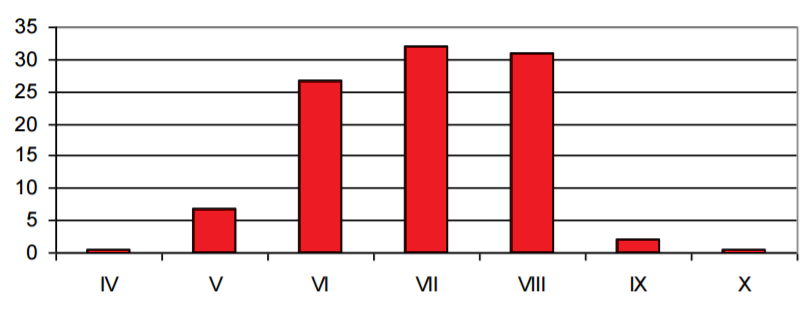
\includegraphics[scale=0.6]{./pictures/r_factor_graph.png}
      \caption[Rozdělení faktoru R během vegetačního období]{Rozdělení
        faktoru R během vegetačního období [\%] dle
        \cite{janecek2012}}
      \label{fig:r_faktor_graph}
\end{figure}
\vspace{-16pt} Faktor C vyjadřuje poměr smyvu z pozemku chráněném
pěstovanou plodinou ku~smyvu na pozemku, jež je udržován jako úhor,
kypřený po každém dešti. Nejlepší metodou je zjištění struktury
plodin, osevních postupů a metodiky hospodaření od~zemědělského
subjektu užívajícího daný pozemek.

Pro určení vegetačního faktoru lze též využít Protierozní
kalkulačku\cite{kalkulacka}, která po vybrání příslušného osevního
postupu zobrazí C faktor pro celé období postupu.  Pokud to není
možné, lze využít průměrné zastoupení plodin a vypočítat C faktor jako
vážený průměr z hodnot uvedených v tabulce \ref{tabulka_c}.
\begin{table}[!h]
\begin{center}
\catcode`\-=12
    \noindent\begin{tabular}{|*{4}{c|}} \hline \bf Plodina & \bf C &
    \bf Plodina & \bf C\\ \hline \bf pšenice ozimá &0,12 &\bf
    chmelnice &0,80\\ \hline \bf žito ozimé &0,17 &\bf řepka ozimá
    &0,22\\ \hline \bf ječmen jarní &0,15 &\bf slunečnice
    &0,60\\ \hline \bf ječmen ozimý &0,17 &\bf mák &0,50\\ \hline \bf
    oves &0,10 &\bf ostatní olejniny &0,22\\ \hline \bf kukuřice na
    zrno&0,61 &\bf kukuřice na siláž &0,72\\ \hline \bf luštěniny
    &0.05 &\bf ostatní pícniny - jednoleté&0,02\\ \hline \bf brambory
    rané &0.60 &\bf ostatní pícniny - víceleté &0,01\\ \hline \bf
    brambory pozdní &0.44 &\bf zelenina &0,45\\ \hline \bf louky
    &0,005 &\bf sady &0,45\\ \hline
    \end{tabular}\\
  \caption[Hodnoty C faktoru pro jednotlivé plodiny]{Hodnoty C faktoru
    pro jednotlivé plodiny dle metodiky \cite{janecek2012}.}
  \label{tabulka_c}
\end{center}
\end{table}
\FloatBarrier
\subsection{Faktor protierozních opatření (P)}
Při využití agrotechnických metod protierozní ochrany, jako jsou
konturové obdělávání, pásové střídání plodin, hrázkování či
terasování, je snižován faktor P. Důležité ovšem je dodržet podmínky
maximálních délek a počtu pásů, jinak musí být volena základní hodnota
P faktoru, tedy $P=1$.

Přehled všech metod a hodnot P faktoru lze najít v USLE\cite{usle1978}
nebo Janečkově metodice\cite{janecek2012}.

\subsection{Přípustná průměrná dlouhodobá ztráta půdy ($G_P$)}
Dle vypočteného faktoru G lze rozdělit potenciální ohrožení půdy do 6
kategorií.\cite{vumop}

\begin{table}[!h]
\begin{center}
\catcode`\-=12
    \noindent\begin{tabular}{|*{3}{c|}} \hline \bf Kategorie & \bf
    $\bf G~(t\cdot ha^{-1}\cdot rok^{-1})$ & \bf Kategorie ohroženosti
    vodní erozí\\ \hline 1 & méně než 1,0 & velmi slabě
    ohrožená\\ \hline 2 & 1,1 - 2,0 & slabě ohrožená\\ \hline 3 & 2,1
    - 4,0 & středné ohrožená\\ \hline 4 & 4,1 - 8,0 & silně
    ohrožená\\ \hline 5 & 8,1 - 10,0 & velmi silně ohrožená\\ \hline 6
    & více než 10,1 & extrémně ohrožená\\ \hline
    \end{tabular}\\
  \caption[Rozdělení potenciální ohroženosti půdy]{Rozdělení
    potenciální ohroženosti půdy dle VÚMOP \cite{vumop}.}
  \label{tabulka_ohrozenost}
\end{center}
\end{table}
\FloatBarrier Pro dlouhodobé zachování výrobních, ale i nevýrobních,
funkcí půdy je definována přípustná průměrná roční ztráta, která by
neměla být překročena. Pokud k tomu na pozemku dojde, je třeba zvolit
účinnější protierozní postupy. Hodnota faktor dlouhodobé ztráty půdy
se odvíjí od hloubky půdy, tu lze kromě terénního měření určit rovněž
z 5. číslice kódu BPEJ.\cite{janecek2012}

Mělké půdy (čísla 5 a 6) je doporučeno zatravnit, případně
zalesnit. Kromě půd s kódem 8 a 9, pro které je třeba hloubku půdy
potřeba zjistit terénním průzkumem, je pro ostatní půdy přípustná
hodnota $G_P=4,0~t\cdot ha^{-1}\cdot rok^{-1}$.\cite{Novotny2014}
\newpage
\chapter{Podklady}
V této kapitole jsou popsány mapové podklady využívané při výpočtu 
faktorů pro USLE. V České republice se jedná zejména o vrstvy 
BPEJ~($K, G_P$), LPIS~($C$) a DMT($LS$).
\section{BPEJ}
Prvním krokem k vytvoření systému hodnocení půdy BPEJ bylo v roce 1961
zahájení celosvětově ojedinělého Komplexního průzkumu půd(KPP), při
kterém bylo odebráno okolo 700~000~ půdních sond, ze kterých byly
zpracovány mapové podklady. Na základě nichž byl v roce 1971 začala
tvorba systému ocenění zemědělské půdy - proběhla tzv.~Bonitace
zemědělského půdního fondu.

Původní mapy 1~:~5000 byly zvektorizovány do bonitačního informačního
systému, který je průběžně aktualizován a zpřesňován. Přehled všech
informací o BPEJ je dostupný v eKatalogu BPEJ od
VÚMOP\cite{bpej_vumop}. Ke 3.4.2017 Státní pozemkový úřad uvolnil
celostátní databázi volně ke stažení ve formátu Esri Shapefile\cite{spucr}.
\begin{figure}[H]
    \centering
    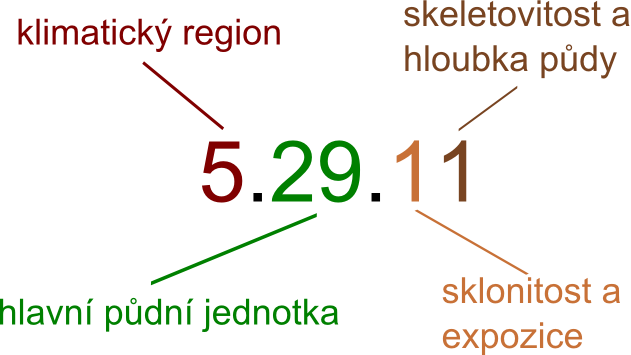
\includegraphics[scale=0.5]{./pictures/Struktura_BPEJ.png}
      \caption[Struktura kódu BPEJ]{Struktura kódu BPEJ, zdroj:
        VÚMOP\cite{bpej_vumop}}
      \label{fig:struktura_bpej}
\end{figure}
Bonitovaná půdně ekologická jednotka je vyjádřena pětimístným kódem ve
formátu - X.XX.XX. Kdy první číslice určuje příslušící klimatický
region(0-9). Druhá a třetí zařazuje půdu do hlavní půdní
jednotky(HPJ)(01-78), pomocí které je ve většině případů možné určit K
faktor~(viz. tab.\ref{hpj_k}). Čtvrtá číslice vymezuje kombinaci
sklonitosti a expozice svahu ke světovým stranám(0-9). Pátá číslice
určuje kombinaci skeletovitosti půdního profilu s hloubkou půdy(0-9),
tato číslice je využívána pro získání hloubky půdy při určení
$G_P$.\cite{Novotny2013}
\section{LPIS}
\begin{figure}[H]
    \centering 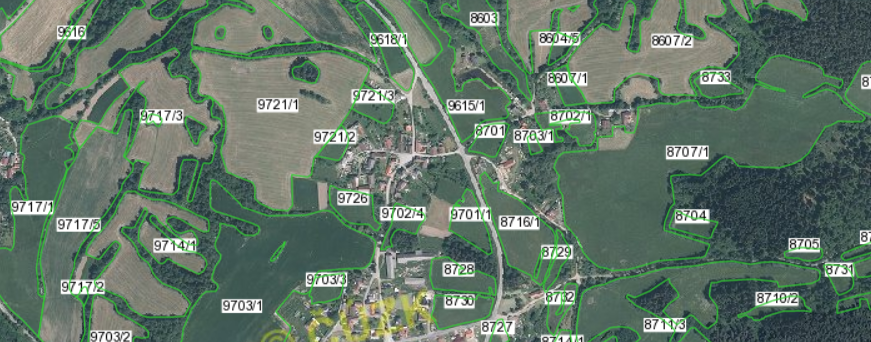
\includegraphics[scale=0.7]{./pictures/lpis.png}
      \caption[Ukázka GIS online aplikace Registr půd]{Ukázka online
        GIS aplikace Registr půd, zdroj: Registr půd\cite{lpis}}
      \label{fig:lpis}
\end{figure}
V roce 1999 se Česká republika zavázala vybudovat do vstupu do EU
systém evidence půdy, který bude založený na uživatelských
vztazích. Jelikož takový systém v ČR do té doby nebyl, tak první verze
z roku 2002 vznikla zakreslením půdních bloků z leteckých snímků do
offline geografického informačního systému, tyto bloky byly následně
schváleny příslušnými uživateli půdy. Toto první řešení bylo v roce
2004 nahrazeno online aplikací Registr půdy\cite{lpis}, která
usnadnila přístup k materiálům LPIS. Ty lze z Registru půdy exportovat
pro vybrané území.\cite{lpis}

Při výpočtu USLE se LPIS využívá k rozdělení na jednotlivé erozně
uzavřené celky(EUC) neboli pozemky, na kterých je eroze počítána. Dále
může být využito rozdělení pozemků dle kultur, pomocí kterého je možné
určit zakládní C faktor a~stanovit pozemky s ornou půdou, pro které je
třeba zjistit pěstované plodiny.\cite{Novotny2014}
\begin{table}[!h]
\begin{center}
\catcode`\-=12
    \noindent\begin{tabular}{|*{3}{c|}} \hline \bf Kód & \bf Kultura &
    \bf C faktor\\ \hline R & orná půda & dle pěstované
    plodiny\\ \hline C & chmelnice & 0,8\\ \hline V & vinice &
    0,4\\ \hline S & ovocný sad & 0,45\\ \hline T & travní porost &
    0,005\\ \hline L & zalesněno & 0,003-0,009\\ \hline O & jiná
    kultura & nutno určit kulturu\\ \hline
    \end{tabular}\\
  \caption[Rozdělení kultur na zemědělské půdě dle LPIS]{Rozdělení
    kultur na zemědělské půdě dle LPIS\cite{lpis} s C faktory
    dle\cite{janecek2012}.}
  \label{tabulka_ohrozenost}
\end{center}
\end{table}
\FloatBarrier
\section{DMT}
%%% ML: nejaky obrazek/screenshot?
%%% RN: Idealne bych chtel vlozit porovnani 4G/5G, zatim jsem
%       nenasel nic vhodneho.
Pro výpočet LS faktoru se v ČR při využití GIS používají především
digitální model reliéfu vytvořenými ČÚZK\cite{cuzk}. Výpočty nad
DMR~4G jsou rychlejší díky pravidelné mřížce, zatímco výpočty nad
DMR~5G poskytují přesnější model terénu.
\subsection{DMR 4G}
%%% ML: Zbytecne dlouha veta
%%% RN: Rozdelil jsem ji na dve
Digitální model reliéfu České republiky 4.~generace~(DMR~4G)
vznikl leteckým laserovým skenováním v letech 2009 až 2013. DMR~4G 
zobrazuje přirozený nebo lidskou činností upravený zemský povrch v 
pravidelné síti 5~x~5~m, která je tvořena body s~určenou nadmořskou
výškou~(Bpv). Pro tento model byla vypočtena úplná střední chyba výšky
0,3~m v odkrytém terénu a 1~m v zalesněném terénu.
\subsection{DMR 5G}
Pro vytvoření páté generace digitálního modelu terénu byla použita
stejná data jako pro čtvrtou generaci. DMR~5G se tedy od předchozího
DMR~4G liší především použitím nepravidelné trojúhelníkové bodové
sítě~(TIN). Tím bylo dosaženo nižší úplné střední chyby výšky a to
0,18~m v odkrytém terénu a 0,3~m v zalesněném terénu.
